\chapter{Developing the solution}

% Ada, Berners-Lee, Cerf, Dijkstra, Engelbart, Flowers, Gates, Hassabis, Ito, Jobs

\section{Sprint Ada}

This is Sprint Ada, the first iteration of my program. This iteration will be terminal-based, and mainly for creating the BFS implementation and adding in relevant functionality such as being able to enter multiple points, a basic visualisation etc.

\subsection{Tasks}

\begin{table}[htbp]
\centering
\begin{tabularx}{\textwidth}{|l|X|}
\hline
\textbf{Task ID} & \textbf{Task Description} \\
\hline
OCSP-001 & BFS Initialisation: Compare the representation methods available for BFS and then find a way to program that representation into the first version of the program. Main focus on a CLI and only 2 points \\
\hline
OCSP-002 & Terminal Visualisation: Create a basic visualisation of a path between 2 points in the terminal\\
\hline
OCSP-003 & Multi-point entry: Allow user to enter more than 2 points and find the shortest path between each, forming a large path from start to end. \\
\hline
\end{tabularx}
\end{table}

\subsection{Purpose}

This sprint entails me creating the first, basic algorithm for the SPA feature, and adding the multi-point entry so that it is useful in this scenario, as I intend for multiple items to be picked up at once.


\clearpage
\subsection{Sprint Planning Details}

\subsubsection{Technical Approach}

As this is still a very basic program and is in the alpha stages of development, this prototype will start with procedural programming, and once the main BFS features have been confirmed to work in the first few iterations, I will move to an object-oriented approach. (OCSP-001)
\begin{enumerate}
    \item Create a 10 $\times$ 10 2D array to represent the graph.
    \item Define the start and end nodes.
    \item Initialize the queue with the start node.
    \item Create an empty set for visited nodes.
    \item Define possible movement directions (up, down, left, right).
    \item While the queue is not empty:
        \begin{enumerate}
            \item Pop the first path from the queue.
            \item Get the last node in the current path.
            \item If the last node is the end node, return the current path.
            \item If the last node has not been visited, mark it as visited.
            \item For each possible direction:
                \begin{enumerate}
                    \item Calculate the new node.
                    \item If the new node is within bounds and not visited:
                        \begin{itemize}
                            \item Create a new path including the new node
                            \item Add the new path to the queue
                        \end{itemize}
                \end{enumerate}
        \end{enumerate}
    \item Create a function to repeat the pathfinding process for all points the user defines to find the shortest path between each pair of nodes. (OCSP-003)
    \item Display the path in a pretty format. (OCSP-002)
\end{enumerate}



\subsubsection{Architecture \& Structural Considerations}

Below are the data structures I plan to use.
\begin{itemize}
    \item 2D Array (List of Lists): The graph is represented as a 10 x 10 2D array (list of lists in Python), where each element can be either 0 (indicating a free cell) or 1 (indicating an obstacle).
    \item Queue: A list is used to implement the queue for BFS, where paths are stored and processed in a first-in, first-out (FIFO) manner.
    \item Set: A set is used to keep track of visited nodes to avoid processing the same node multiple times.
    \item List: Lists are used to store paths and directions.

\end{itemize}

\subsubsection{Dependencies}
There are no dependencies as such currently, I have opted to use Python's built-in functions (namely the list) for the queue rather than the external library \verb|queue|. This may change in future iterations if the code becomes too complex.

\subsection{Development Summary}

\subsubsection{Iteration 1 - Hours: 3}
\begin{itemize}
    \item \textbf{Progress made:}
    \begin{itemize}
        \item OCSP-001: Created a fully working implementation of BFS that outputs the path it took, tested on a simple 10x10 grid.
        \item OCSP-002: Came up with an approach on how to output the path in a more interactive format, similar to the interface I presented in the usability section (see section X.X.X). I plan to use placeholder characters in the array to interpret the terminal output, as colours are not supported in most terminal emulators. [*] represents a user input point, and [=] represents the path taken.
    \end{itemize}
    \item \textbf{Blockers identified:}
    \begin{itemize}
        \item I used my knowledge from the CS50AI course to create the basic BFS implementation between 2 points. However, I struggled to think about how I could implement multiple points.

    \end{itemize}
    \item \textbf{Plan for next day:}
    \begin{itemize}
        \item Find a way to calculate the shortest path between more than 2 points.
        \item Add the visualisations using placeholder characters.
    \end{itemize}
\end{itemize}

\subsubsection{Iteration 2 - Hours: 1.5}
\begin{itemize}
    \item \textbf{Progress made:}
    \begin{itemize}
        \item OCSP-002: I completed the visualisation using my placeholder characters, displaying a grid in the terminal.
        \item OCSP-003: I managed to come up with an approach where the BFS algorithm is run between each pair of points, and the path is then connected together.
    \end{itemize}
    \item \textbf{Blockers identified:}
    \begin{itemize}
        \item I found that the grid did not display correctly as the user could not differentiate between their chosen points and the path followed. This was a very quick fix of highlighting user points AFTER the path was formed, overwriting the path syntax with the point syntax.

    \end{itemize}
\end{itemize}

% Repeat daily log format for each development day

\clearpage
\subsection{Sprint Ada Implementation}

\subsubsection{Iteration 1: The BFS algorithm}

\textbf{Code Changes:}
\begin{itemize}
    \item \textbf{GitHub Commit(s):} d2fe05e, ad6ff95, e2c67a46
    \item \textbf{Modular Structure:}
    \begin{itemize}
        \item I enclosed the BFS algorithm in a function called \verb|bfs| with the parameters \verb|graph_in|, \verb|start| and \verb|end|. I originally intended to use consistent names, however Qodana flagged that this is not conventional. The naming scheme would have been in violation of PEP 3104, which addressed this issue. As such, I changed variable names like \verb|graph| to \verb|graph_in|, which is still an appropriate name (as it refers to the parameter being passed INto the function) but does not violate Python conventions.
        \item I chose a basic function structure for now, as I have only made a small part and single feature of my solution. However, I did implement sub-programs to organise my code better and allow for better debugging.
    \end{itemize}
\end{itemize}

\textbf{Code Quality:}
\begin{itemize}
    \item \textbf{Annotations added:} As I was planning to continue this at a later time, I annotated each step of the BFS algorithm so that I could easily backtrack and visualise what was happening. I annotated most lines to ensure I would understand exactly how the algorithm worked and I could dry-run the algorithm in my head.
    \item \textbf{Variable/Structure naming:} I followed the lower-case underscore convention as defined by PEP 8. I focused on using industry terminology as my variable names, for example \verb|path| and \verb|node| 
    \item \textbf{Modular approach:} I have encapsulated all BFS-related code in a single BFS function. I have opted for this approach as BFS is a relatively simple algorithm, meaning the code is quite short and is appropriate to group into a single function.
\end{itemize}

\newpage

\subsubsection{Code Implementation:}
\begin{verbatim}
rows, cols = 10, 10
graph = [[0 for _ in range(cols)] for _ in range(rows)]

def bfs(graph_in, start, end):
    queue = [[start]] # Start with the start node
    visited = set() # Keep track of visited nodes
    directions = [(-1, 0), (1, 0), (0, -1), (0, 1)]  # Up, Down, Left, Right

    while queue:
        path = queue.pop(0) # Get the first path in the queue
        x, y = path[-1] # Get the last node in the path

        if (x, y) == end:
            return path # Return the path if we reach the end

        if (x, y) not in visited: # If the node has not been visited
            visited.add((x, y))  # Mark the node as visited
            for dx, dy in directions:  # Check all possible directions
                nx, ny = x + dx, y + dy  # Calculate the new node
                if 0 <= nx < rows and 0 <= ny < cols:  
                # Check if the new node is within the bounds
                    if (nx, ny) not in visited: 
                    # Check if the new node is not visited
                        new_path = list(path) + [(nx, ny)]  # Add new node to path
                        queue.append(new_path) # Add new path to queue

    return None  # Return None if no path is found


start_node = (0, 0)
end_node = (4, 8)

path = bfs(graph, start_node, end_node)
print(path)

\end{verbatim}

\newpage

\begin{figure}[htbp!]
    \centering
    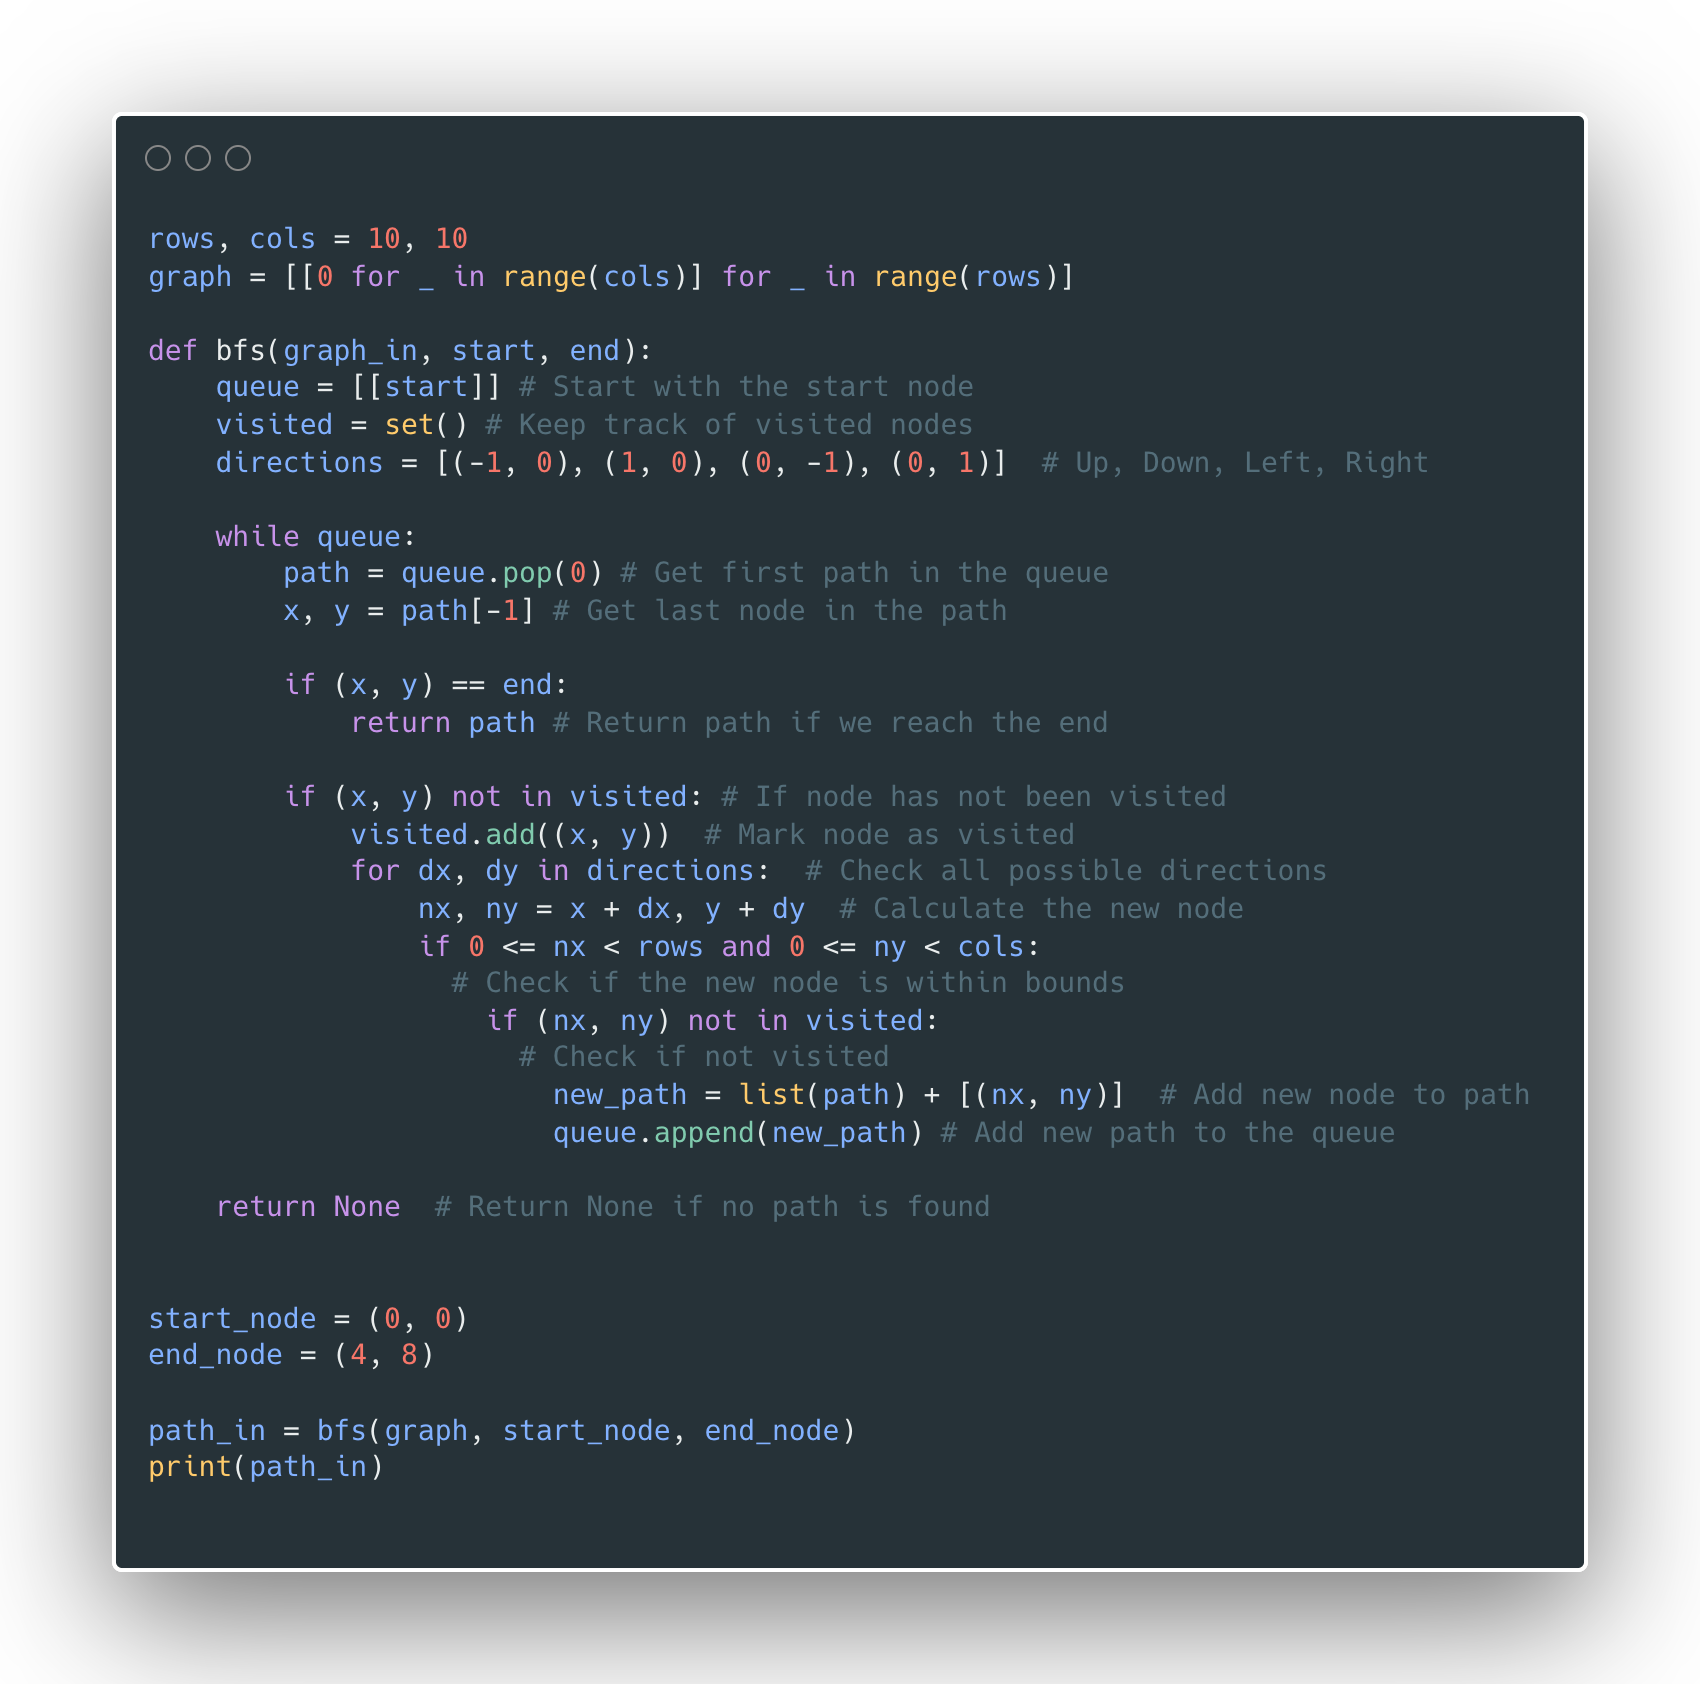
\includegraphics[width=1\linewidth]{Images/Source Code Image (2).png}
    \caption{A coloured screenshot of the code}
\end{figure}
\textbf{}\newline
\newpage

\subsubsection{Prototype Version:} 
Currently, the BFS algorithm is working well for 2 defined points: a start and end node. It outputs a basic list of the coordinates that were followed to reach the end node from the start node. However, there is no visualisation as of yet, this will be implemented in the next iteration after some planning. As well as this, the BFS algorithm can currently handle only 2 points at a time, therefore I will be researching into how I can implement more points and allow the user to be able to set points to stop at.
\begin{figure}[htbp]
    \centering
    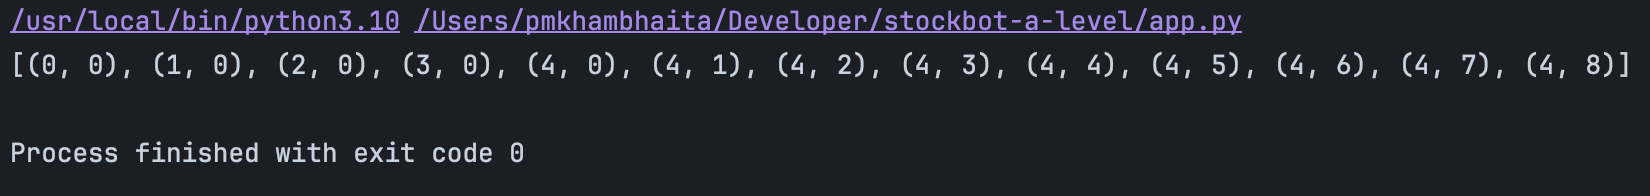
\includegraphics[width=0.8\textwidth]{Images/Screenshot 2025-03-30 at 11.18.52.png}
    \caption{The output of my algorithm with start at (0,0) and end at (4,8)}
\end{figure}

\subsubsection{Testing:}
\begin{table}[htbp]
\centering
\begin{tabularx}{\textwidth}{|l|X|p{3.5cm}|p{3.5cm}|c|}
\hline
\textbf{ID} & \textbf{Description} & \textbf{Expected} & \textbf{Actual} & \textbf{Pass?} \\
\hline
T1.1 & Input 0,0 and 9,9 & Direct path between both points & Direct path between points & X \\
\hline
T1.2 & Input 1,2 and 5,7 & Direct path between defined points only & Direct path between 1,2 and 5,7 & X \\
\hline
T1.3 & Input -1,-1 and 4,8 & Returns error & Error and break & \~{} \\
\hline
T1.4 & Input 0,1 and 10,10 & Return error & Error and break & \~{} \\
\hline

\end{tabularx}
\caption{Testing results for iteration 1}
\end{table}
\textbf{}\newline
T1.1 and T1.2 were successful, meaning the core functionality of the program is functional as expected. However, T1.3 and T1.4 were partially successful. While I did include the validation, I did not add a graceful error message, it was left to the basic python error-catching mechanisms. This will be fixed in the next iteration.

\newpage

\subsubsection{Screenshots of tests/program}

\begin{figure}[htbp!]
    \centering
    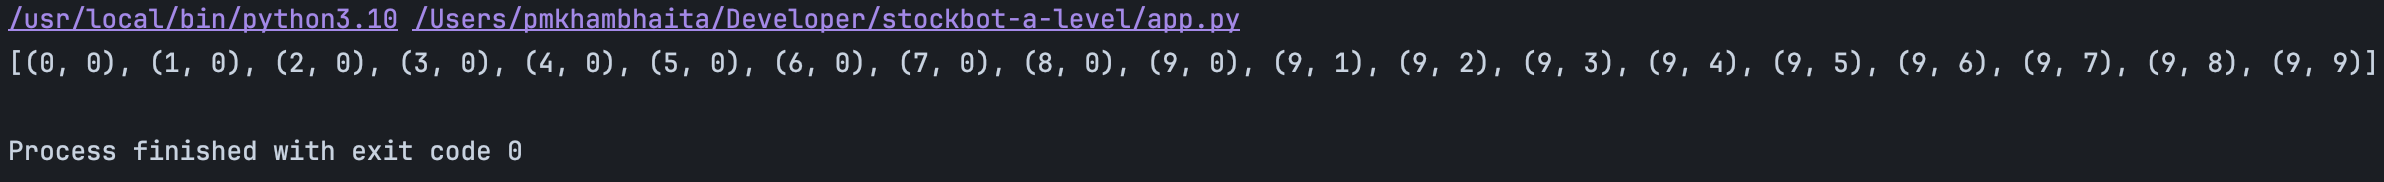
\includegraphics[width=1\linewidth]{Images/t1.1.png}
    \caption{T1.1 Output}
    \label{fig:enter-label}
\end{figure}

\begin{figure}[htbp!]
    \centering
    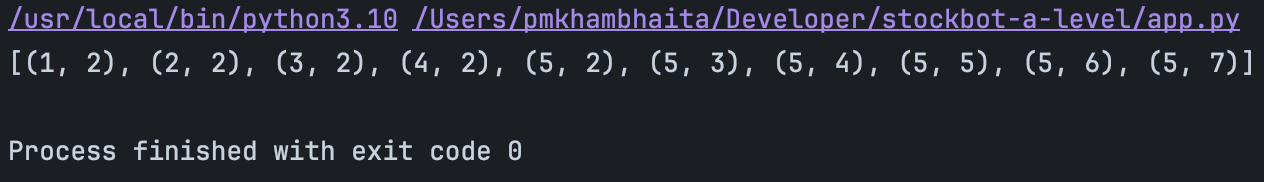
\includegraphics[width=1\linewidth]{Images/t1.2.png}
    \caption{T1.2 Output}
    \label{fig:enter-label}
\end{figure}

\begin{figure}[htbp!]
    \centering
    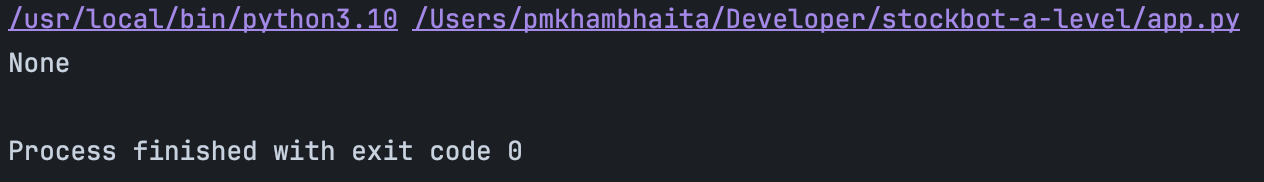
\includegraphics[width=1\linewidth]{Images/t1.3,1.4.png}
    \caption{T1.2 Output}
    \label{fig:enter-label}
\end{figure}

\begin{figure}[htbp!]
    \centering
    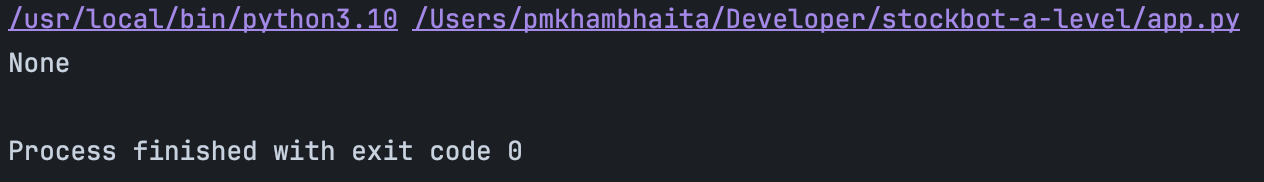
\includegraphics[width=1\linewidth]{Images/t1.3,1.4.png}
    \caption{T1.2 Output}
    \label{fig:enter-label}
\end{figure}

\newpage

\subsubsection{Validation:}
\begin{itemize}
    \item Boundary check: I ensured that the new node \verb|(nx, ny)| is within the bounds of the graph
    \item Visited check: I checked that the new node \verb|(nx, ny)| has not been visited before.
\end{itemize}

\subsubsection{Qodana Analysis}
    \begin{itemize}
        \item Issues identified: Shadowed name from outer scope
        \item Resolved issues: Modified variable name to prevent this
    \end{itemize}

\begin{figure}[htbp!]
    \centering
    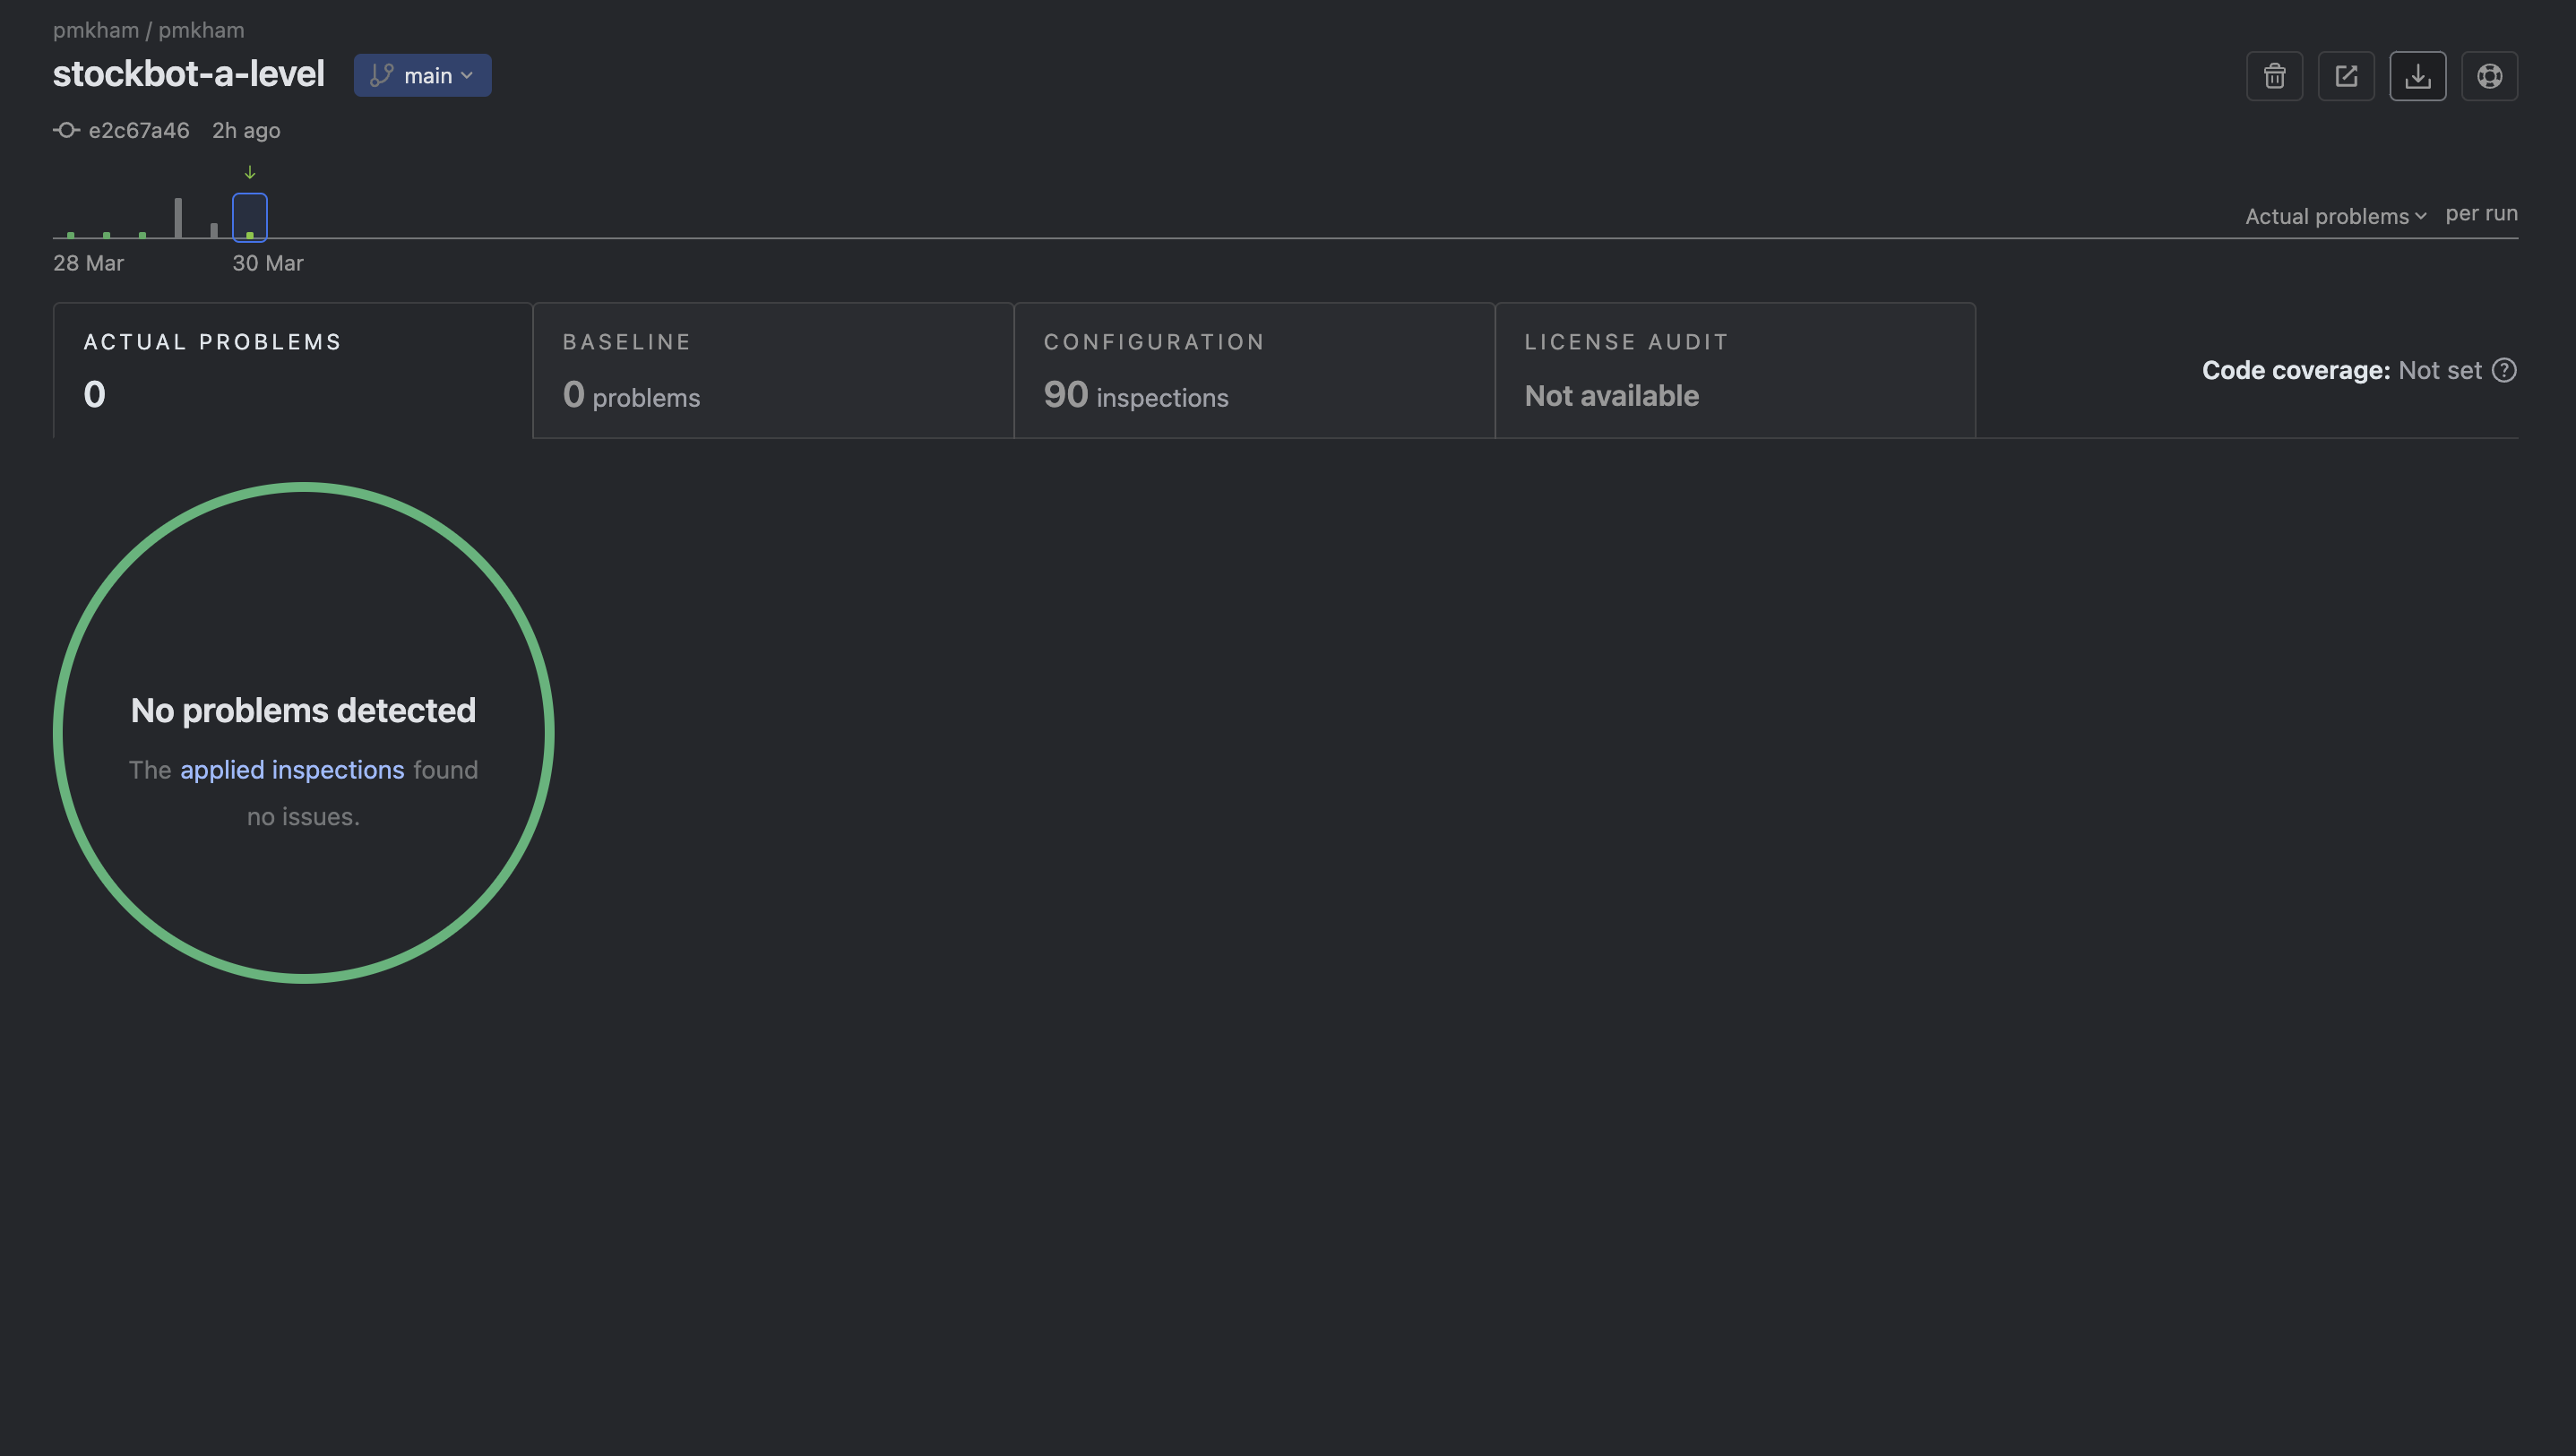
\includegraphics[width=1\linewidth]{Images/qodana-sai1.png}
    \caption{As of commit e2c67a46, no problems were identified.}
\end{figure}

\subsubsection{Review:}
\begin{itemize}
    \item Overall this iteration was quite successful. I managed to get a functional BFS algorithm working between 2 points, however I must be careful in not only validating but adding error messages for specific cases.
    \item Since this is still quite basic, I stuck to a simple procedural format rather than object-oriented principles. In the next iteration, I will be applying object-oriented principles as the program greatens in complexity.
\end{itemize}



\newpage

\subsubsection{Iteration 2: Multi-point BFS and Visualisation}

\textbf{Code Changes:}
\begin{itemize}
    \item \textbf{GitHub Commit(s):} x,x,x
    \item \textbf{Modular Structure:}
    \begin{itemize}
        \item I have now implemented an object-oriented approach to the problem, separating each section into their respective classes. Now that my solution is developing in complexity, I decided to separate the elements of my program further into distinct classes, referencing each other when necessary.
    \end{itemize}
\end{itemize}

\textbf{Code Quality:}
\begin{itemize}
    \item \textbf{Annotations added:} As I was planning to continue this at a later time, I annotated each step of the BFS algorithm so that I could easily backtrack and visualise what was happening. I annotated most lines to ensure I would understand exactly how the algorithm worked and I could dry-run the algorithm in my head.
    \item \textbf{Variable/Structure naming:} I followed the lower-case underscore convention as defined by PEP 8. I focused on using industry terminology as my variable names, for example \verb|path| and \verb|node| 
    \item \textbf{Modular approach:} I have encapsulated all BFS-related code in a single BFS function. I have opted for this approach as BFS is a relatively simple algorithm, meaning the code is quite short and is appropriate to group into a single function.
\end{itemize}

\newpage

\subsubsection{Code Implementation:}
\begin{verbatim}
rows, cols = 10, 10
graph = [[0 for _ in range(cols)] for _ in range(rows)]

def bfs(graph_in, start, end):
    queue = [[start]] # Start with the start node
    visited = set() # Keep track of visited nodes
    directions = [(-1, 0), (1, 0), (0, -1), (0, 1)]  # Up, Down, Left, Right

    while queue:
        path = queue.pop(0) # Get the first path in the queue
        x, y = path[-1] # Get the last node in the path

        if (x, y) == end:
            return path # Return the path if we reach the end

        if (x, y) not in visited: # If the node has not been visited
            visited.add((x, y))  # Mark the node as visited
            for dx, dy in directions:  # Check all possible directions
                nx, ny = x + dx, y + dy  # Calculate the new node
                if 0 <= nx < rows and 0 <= ny < cols:  
                # Check if the new node is within the bounds
                    if (nx, ny) not in visited: 
                    # Check if the new node is not visited
                        new_path = list(path) + [(nx, ny)]  # Add new node to path
                        queue.append(new_path) # Add new path to queue

    return None  # Return None if no path is found


start_node = (0, 0)
end_node = (4, 8)

path = bfs(graph, start_node, end_node)
print(path)

\end{verbatim}

\newpage

\begin{figure}[htbp!]
    \centering
    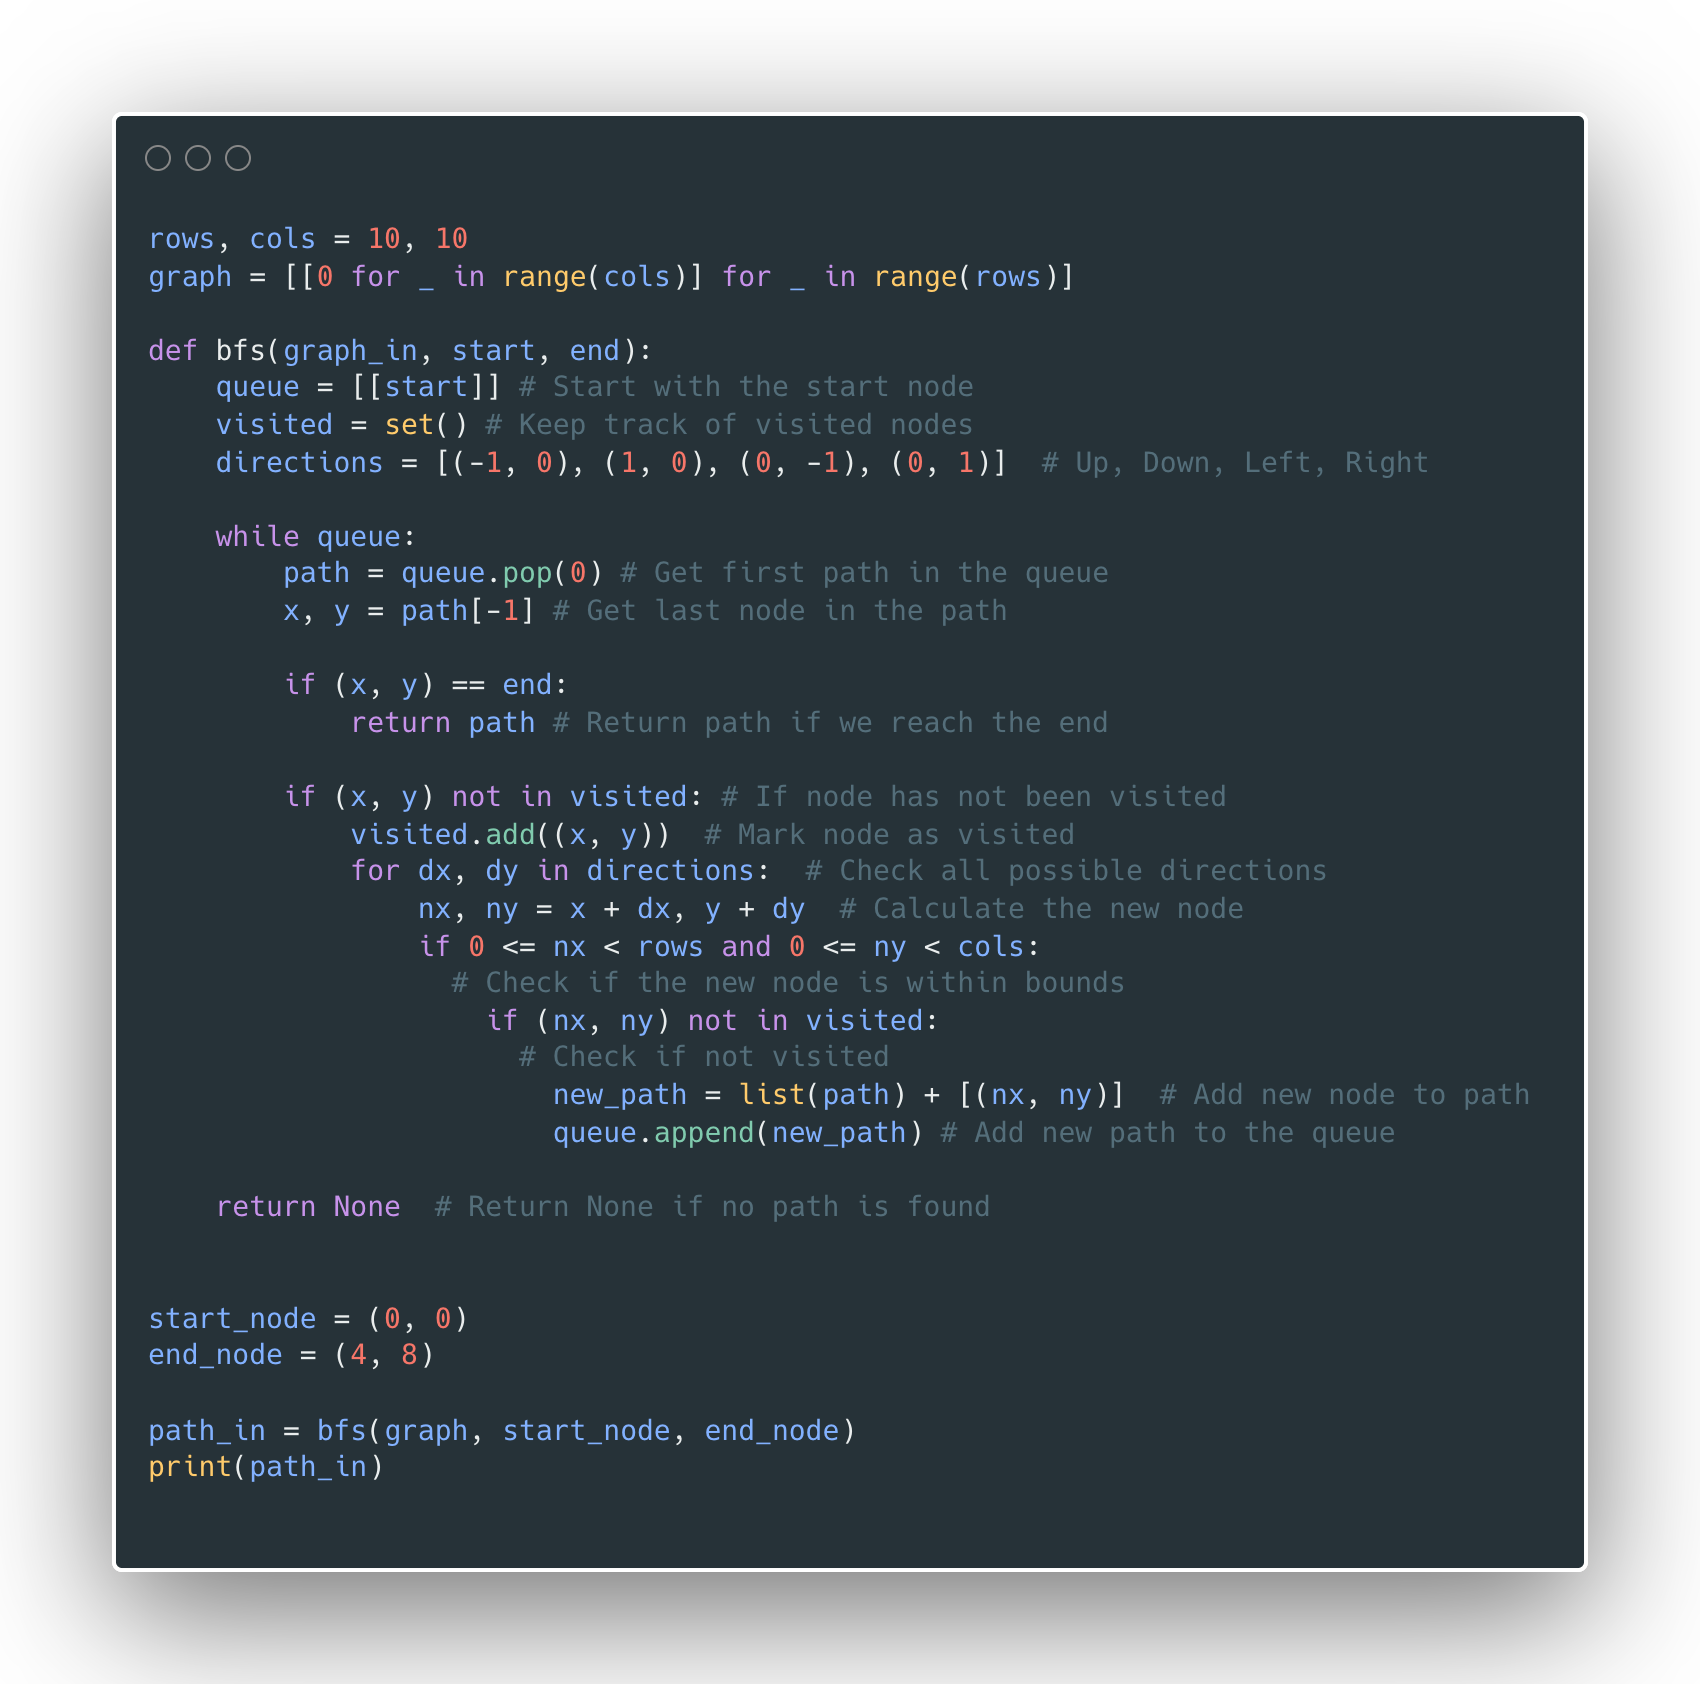
\includegraphics[width=1\linewidth]{Images/Source Code Image (2).png}
    \caption{A coloured screenshot of the code}
\end{figure}
\textbf{}\newline
\newpage

\subsubsection{Prototype Version:} 
Currently, the BFS algorithm is working well for 2 defined points: a start and end node. It outputs a basic list of the coordinates that were followed to reach the end node from the start node. However, there is no visualisation as of yet, this will be implemented in the next iteration after some planning. As well as this, the BFS algorithm can currently handle only 2 points at a time, therefore I will be researching into how I can implement more points and allow the user to be able to set points to stop at.
\begin{figure}[htbp]
    \centering
    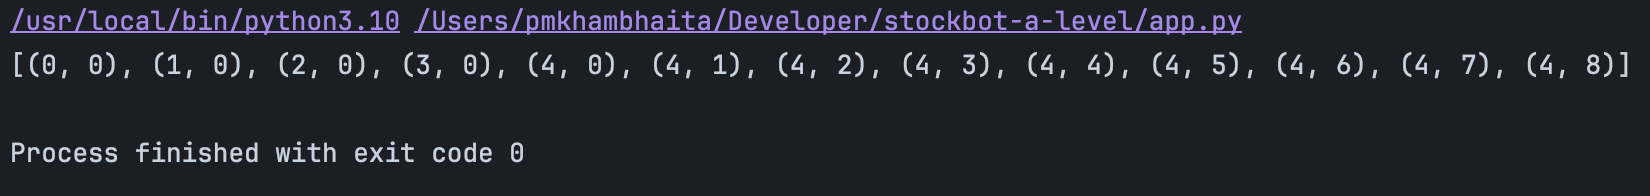
\includegraphics[width=0.8\textwidth]{Images/Screenshot 2025-03-30 at 11.18.52.png}
    \caption{The output of my algorithm with start at (0,0) and end at (4,8)}
\end{figure}

\subsubsection{Testing:}
\begin{table}[htbp]
\centering
\begin{tabularx}{\textwidth}{|l|X|p{3.5cm}|p{3.5cm}|c|}
\hline
\textbf{ID} & \textbf{Description} & \textbf{Expected} & \textbf{Actual} & \textbf{Pass?} \\
\hline
T1.1 & Input 0,0 and 9,9 & Direct path between both points & Direct path between points & X \\
\hline
T1.2 & Input 1,2 and 5,7 & Direct path between defined points only & Direct path between 1,2 and 5,7 & X \\
\hline
T1.3 & Input -1,-1 and 4,8 & Returns error & Error and break & \~{} \\
\hline
T1.4 & Input 0,1 and 10,10 & Return error & Error and break & \~{} \\
\hline

\end{tabularx}
\caption{Testing results for iteration 1}
\end{table}
\textbf{}\newline
T1.1 and T1.2 were successful, meaning the core functionality of the program is working as expected. However, T1.3 and T1.4 were partially successful. While I did include the validation, I did not add a graceful error message, it was left to the basic python error-catching mechanisms. This will be fixed in the next iteration.

\newpage

\subsubsection{Screenshots of tests/program}

\begin{figure}[htbp!]
    \centering
    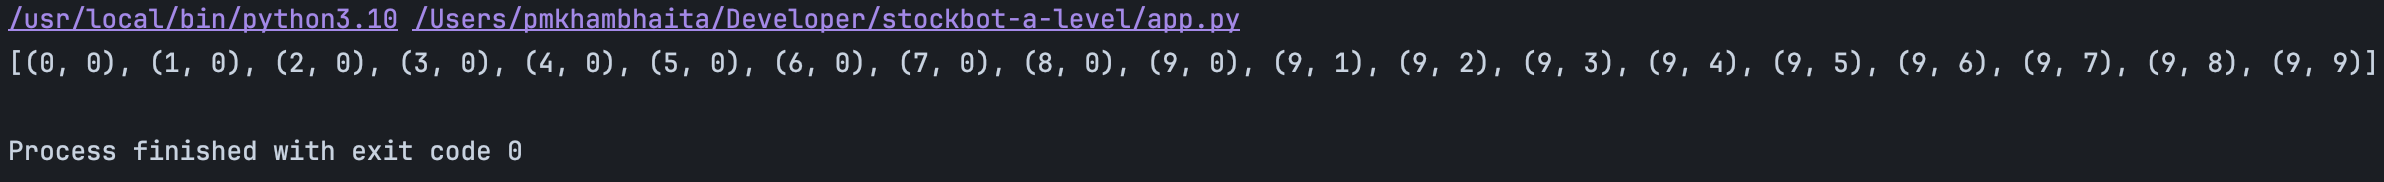
\includegraphics[width=1\linewidth]{Images/t1.1.png}
    \caption{T1.1 Output}
    \label{fig:enter-label}
\end{figure}

\begin{figure}[htbp!]
    \centering
    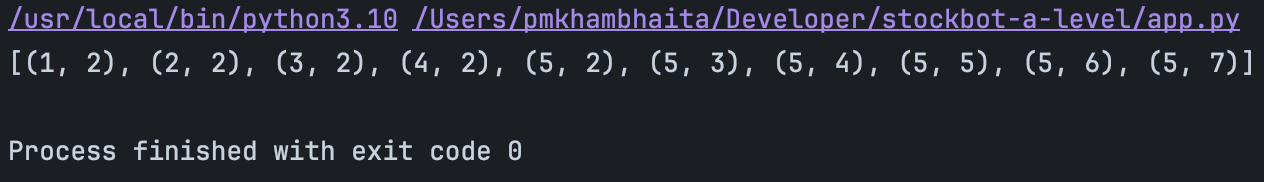
\includegraphics[width=1\linewidth]{Images/t1.2.png}
    \caption{T1.2 Output}
    \label{fig:enter-label}
\end{figure}

\begin{figure}[htbp!]
    \centering
    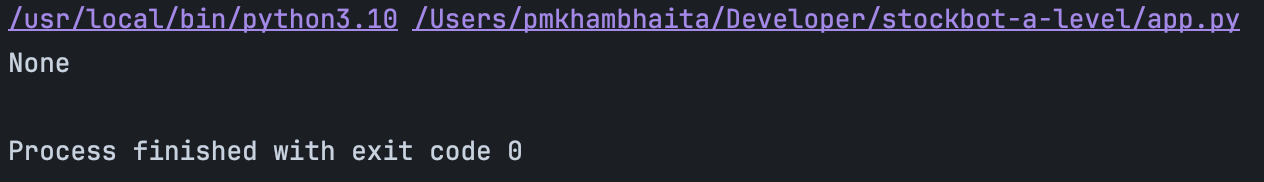
\includegraphics[width=1\linewidth]{Images/t1.3,1.4.png}
    \caption{T1.2 Output}
    \label{fig:enter-label}
\end{figure}

\begin{figure}[htbp!]
    \centering
    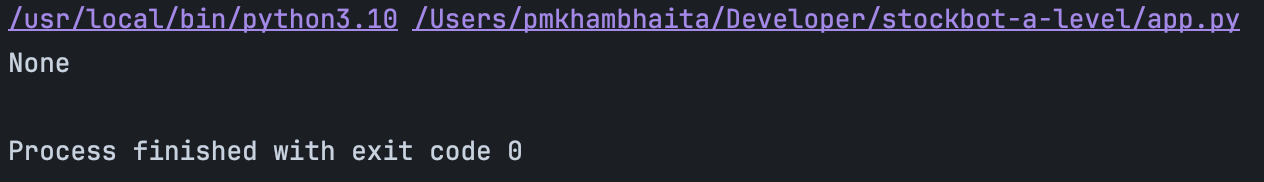
\includegraphics[width=1\linewidth]{Images/t1.3,1.4.png}
    \caption{T1.2 Output}
    \label{fig:enter-label}
\end{figure}

\newpage

\subsubsection{Validation:}
\begin{itemize}
    \item Boundary check: I ensured that the new node \verb|(nx, ny)| is within the bounds of the graph
    \item Visited check: I checked that the new node \verb|(nx, ny)| has not been visited before.
\end{itemize}

\subsubsection{Qodana Analysis}
    \begin{itemize}
        \item Issues identified: Shadowed name from outer scope
        \item Resolved issues: Modified variable name to prevent this
    \end{itemize}

\begin{figure}[htbp!]
    \centering
    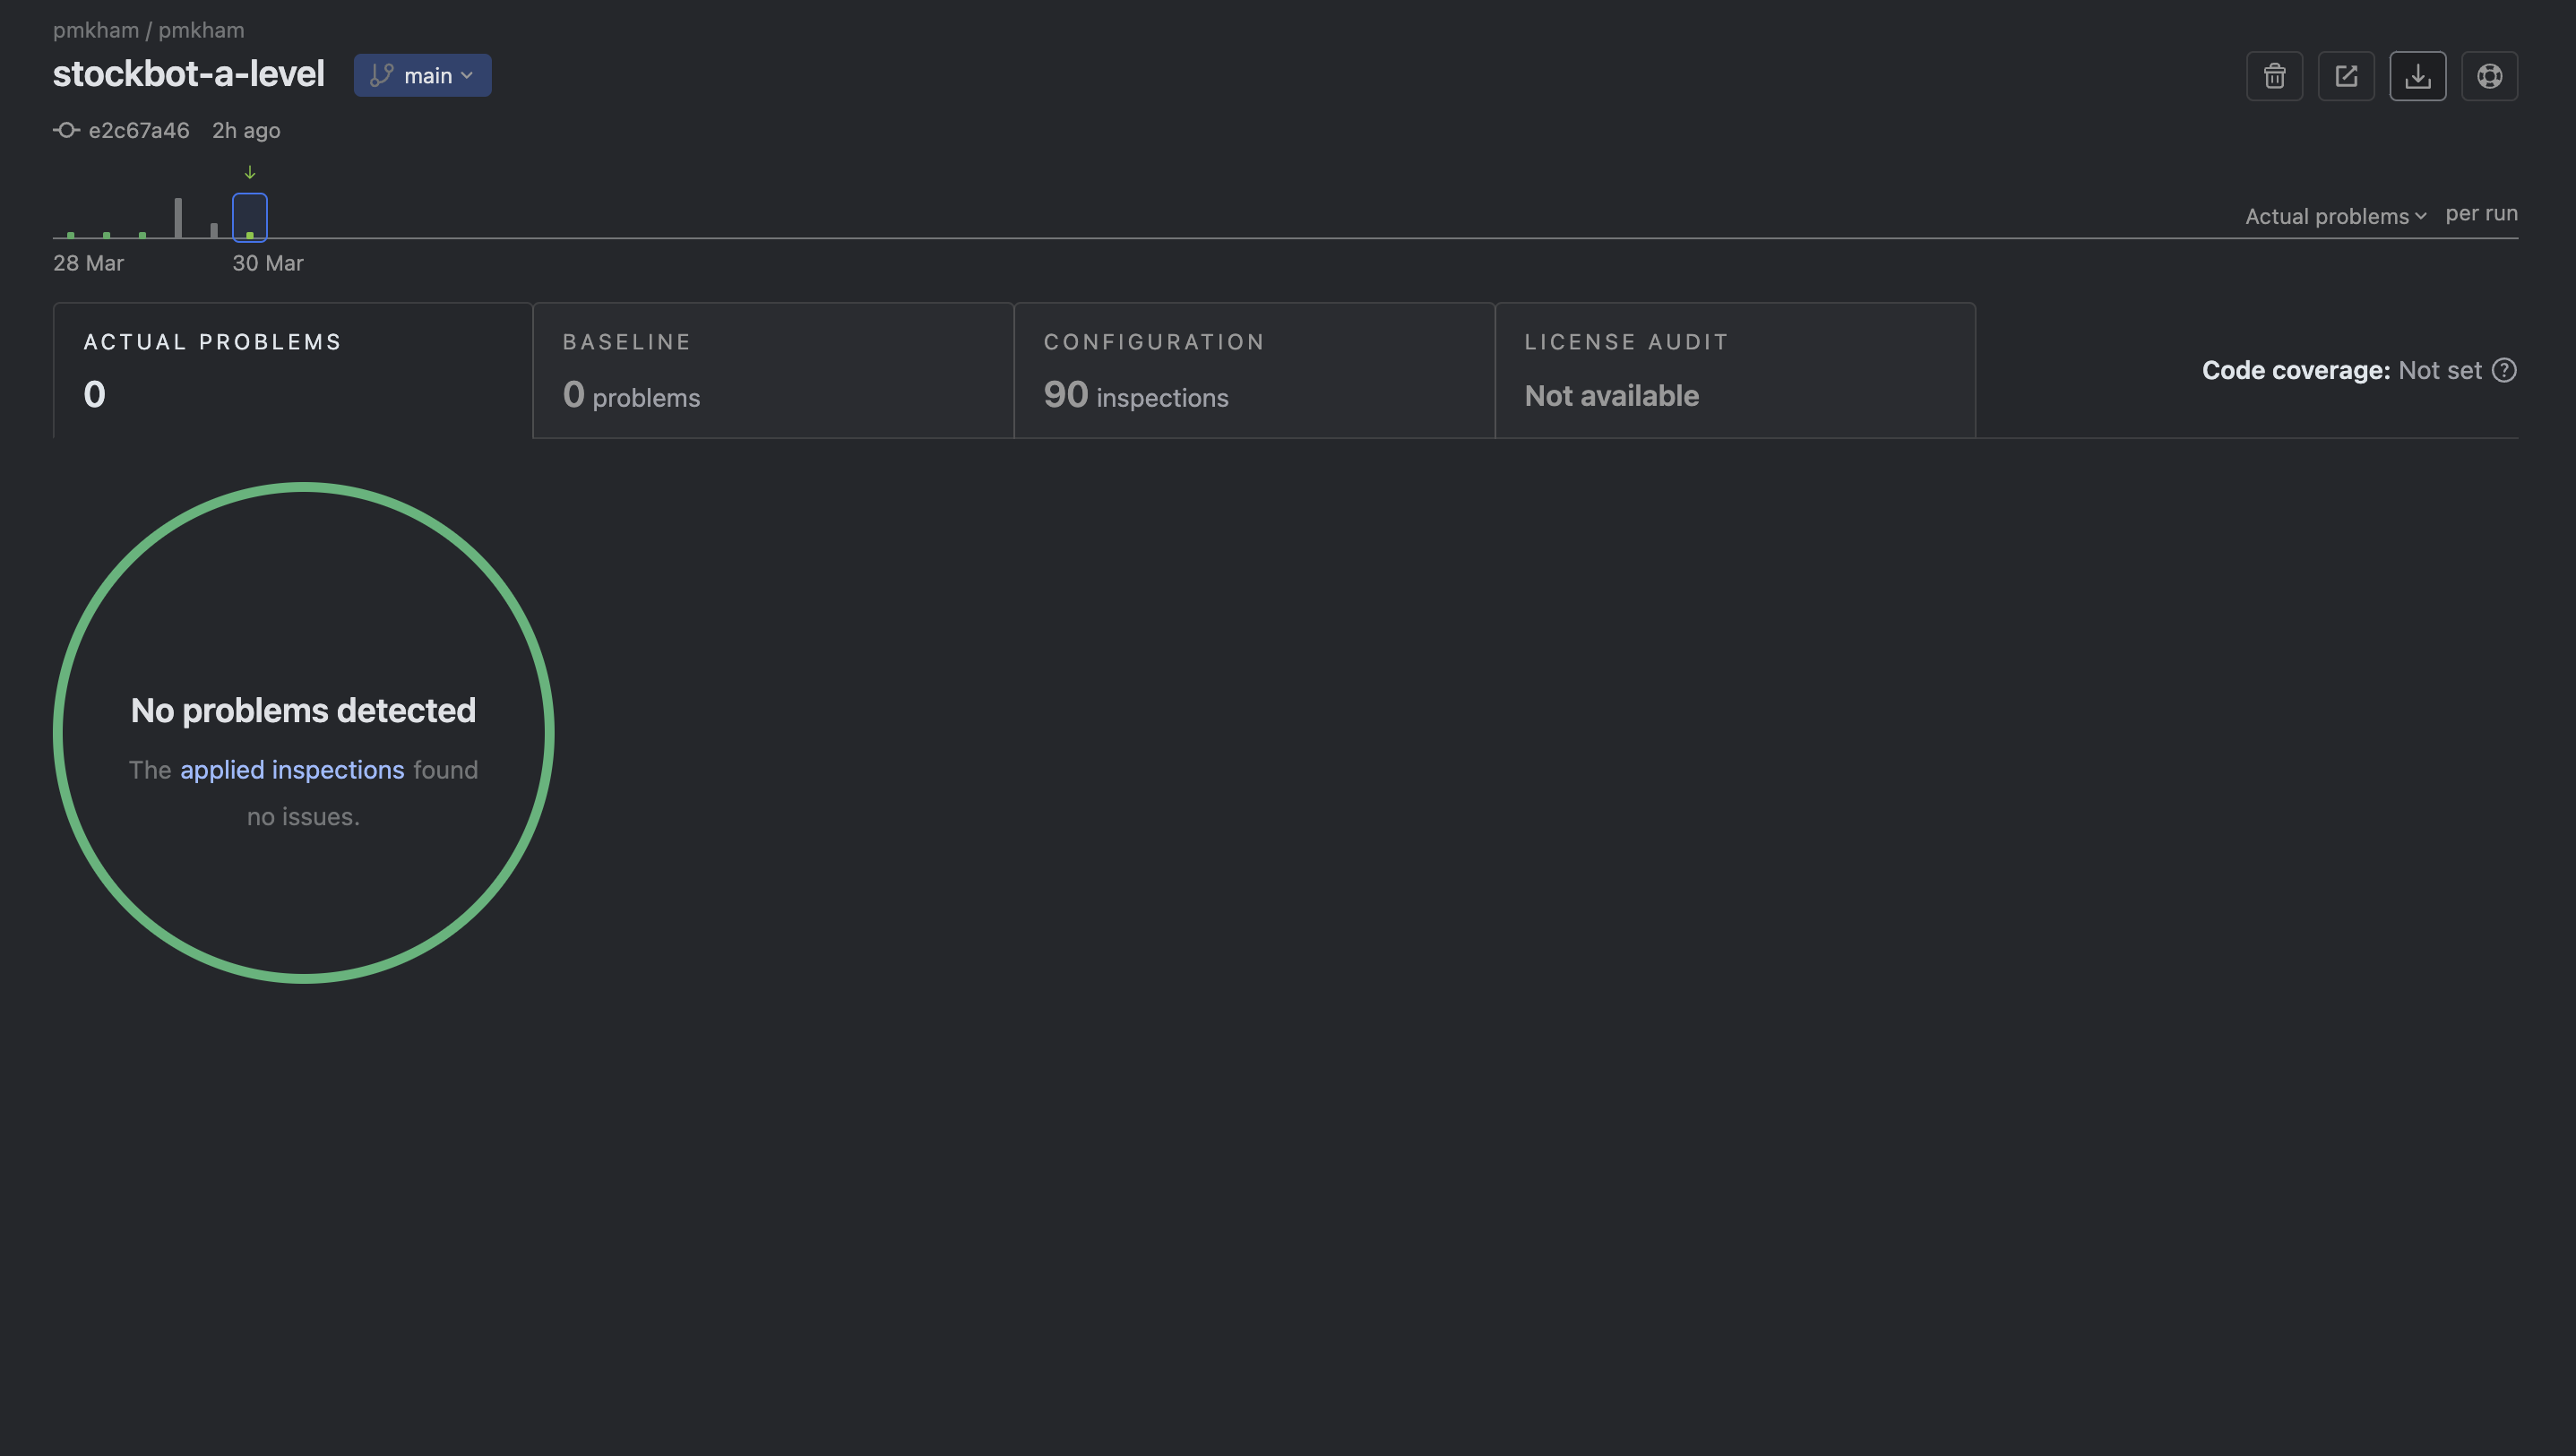
\includegraphics[width=1\linewidth]{Images/qodana-sai1.png}
    \caption{As of commit e2c67a46, no problems were identified.}
\end{figure}

\subsubsection{Review:}
\begin{itemize}
    \item Overall this iteration was quite successful. I managed to get a functional BFS algorithm working between 2 points, however I must be careful in not only validating but adding error messages for specific cases.
    \item Since this is still quite basic, I stuck to a simple procedural format rather than object-oriented principles. In the next iteration, I will be applying object-oriented principles as the program greatens in complexity.
\end{itemize}


\clearpage
\subsection{Sprint Review and Retrospective}

\subsubsection{Accomplishments}
\begin{itemize}
    \item List completed Linear tasks with IDs
    \item Summary of specific features implemented with reference to requirements
\end{itemize}

\subsubsection{Testing Summary}
\begin{table}[htbp]
\centering
\begin{tabular}{|l|c|}
\hline
\textbf{Metric} & \textbf{Count} \\
\hline
Total tests conducted & Number \\
\hline
Tests passed & Number \\
\hline
Tests failed & Number \\
\hline
Fixed issues & Number \\
\hline
\end{tabular}
\caption{Sprint 1 testing summary}
\end{table}

\begin{itemize}
    \item \textbf{Key validation implementations:}
    \begin{itemize}
        \item Describe specific validation techniques implemented
    \end{itemize}
\end{itemize}

\subsubsection{Code Quality Metrics}
\begin{itemize}
    \item \textbf{Qodana final report summary:}
    \begin{itemize}
        \item Specific code quality metrics
        \item List of issues resolved with before/after comparisons
        \item Technical debt measurements
    \end{itemize}
\end{itemize}

\subsubsection{Sprint Review Outcomes}
\begin{itemize}
    \item Specific feedback received
    \item Decisions made for next sprint
\end{itemize}

\subsubsection{Retrospective}
\begin{itemize}
    \item \textbf{What went well:}
    \begin{itemize}
        \item Specific processes or implementations that were successful
    \end{itemize}
    \item \textbf{What could be improved:}
    \begin{itemize}
        \item Specific areas for improvement with technical details
    \end{itemize}
    \item \textbf{Action items for next sprint:}
    \begin{itemize}
        \item Specific technical actions to take in next sprint
    \end{itemize}
\end{itemize}

\clearpage
\subsection{Mark Scheme Alignment Evidence}

\subsubsection{Iterative Development (15 marks potential)}
\begin{table}[htbp]
\centering
\begin{tabularx}{\textwidth}{|l|X|}
\hline
\textbf{Criterion} & \textbf{Evidence Provided} \\
\hline
Stages of iterative process & List specific documentation elements showing all stages \\
\hline
Prototype versions & List all prototype versions with specific features \\
\hline
Modular structure & Describe how code structure demonstrates modularity \\
\hline
Code annotations & Detail annotation approach used for maintenance \\
\hline
Variable naming & Explain naming conventions with examples \\
\hline
Validation approaches & Summarize all validation techniques used \\
\hline
Review stages & List all review points with outcomes \\
\hline
\end{tabularx}
\caption{Evidence for iterative development mark criteria}
\end{table}

\subsubsection{Testing to Inform Development (10 marks potential)}
\begin{table}[htbp]
\centering
\begin{tabularx}{\textwidth}{|l|X|}
\hline
\textbf{Criterion} & \textbf{Evidence Provided} \\
\hline
Testing at each stage & Summarize testing at each iteration with specific tests \\
\hline
Failed tests documentation & Explain how failed tests were documented with examples \\
\hline
Remedial actions & Summarize specific remedial actions taken with justifications \\
\hline
\end{tabularx}
\caption{Evidence for testing mark criteria}
\end{table}

% Repeat the entire section structure for each sprint

\section{Sprint Number: 2}
% Follow the same structure as Sprint 1

\section{Final Solution Review}

\subsection{Solution Overview}
Describe the complete solution with reference to requirements from analysis.

\subsection{Code Structure and Modularity}
Explain the final structure with diagrams if helpful.

\subsection{Key Implementation Features}
Highlight innovative or complex aspects of the solution.

\subsection{Comprehensive Validation Strategy}
Summarize the validation approach across the entire project.

\subsection{Maintenance Considerations}
Explain how the code is designed for future maintenance.

